\documentclass{beamer}
\usepackage{amsmath}
\usepackage[english]{babel} %set language; note: after changing this, you need to delete all auxiliary files to recompile
\usepackage[utf8]{inputenc} %define file encoding; latin1 is the other often used option
\usepackage{csquotes} % provides context sensitive quotation facilities
\usepackage{graphicx} %allows for inserting figures
\usepackage{booktabs} % for table formatting without vertical lines
\usepackage{textcomp} % allow for example using the Euro sign with \texteuro
\usepackage{stackengine}
\usepackage{wasysym}
\usepackage{tikzsymbols}
\usepackage{textcomp}
\newcommand{\bubblethis}[2]{
        \tikz[remember picture,baseline]{\node[anchor=base,inner sep=0,outer sep=0]%
        (#1) {\underline{#1}};\node[overlay,cloud callout,callout relative pointer={(0.2cm,-0.7cm)},%
        aspect=2.5,fill=yellow!90] at ($(#1.north)+(-0.5cm,1.6cm)$) {#2};}%
    }%
\tikzset{face/.style={shape=circle,minimum size=4ex,shading=radial,outer sep=0pt,
        inner color=white!50!yellow,outer color= yellow!70!orange}}
%% Some commands to make the code easier
\newcommand{\emoticon}[1][]{%
  \node[face,#1] (emoticon) {};
  %% The eyes are fixed.
  \draw[fill=white] (-1ex,0ex) ..controls (-0.5ex,0.2ex)and(0.5ex,0.2ex)..
        (1ex,0.0ex) ..controls ( 1.5ex,1.5ex)and( 0.2ex,1.7ex)..
        (0ex,0.4ex) ..controls (-0.2ex,1.7ex)and(-1.5ex,1.5ex)..
        (-1ex,0ex)--cycle;}
\newcommand{\pupils}{
  %% standard pupils
  \fill[shift={(0.5ex,0.5ex)},rotate=80] 
       (0,0) ellipse (0.3ex and 0.15ex);
  \fill[shift={(-0.5ex,0.5ex)},rotate=100] 
       (0,0) ellipse (0.3ex and 0.15ex);}

\newcommand{\emoticonname}[1]{
  \node[below=1ex of emoticon,font=\footnotesize,
        minimum width=4cm]{#1};}
\usepackage{scalerel}
\usetikzlibrary{positioning}
\usepackage{xcolor,amssymb}
\newcommand\dangersignb[1][2ex]{%
  \scaleto{\stackengine{0.3pt}{\scalebox{1.1}[.9]{%
  \color{red}$\blacktriangle$}}{\tiny\bfseries !}{O}{c}{F}{F}{L}}{#1}%
}
\newcommand\dangersignw[1][2ex]{%
  \scaleto{\stackengine{0.3pt}{\scalebox{1.1}[.9]{%
  \color{red}$\blacktriangle$}}{\color{white}\tiny\bfseries !}{O}{c}{F}{F}{L}}{#1}%
}
\usepackage{fontawesome} % Social Icons
\usepackage{epstopdf} % allow embedding eps-figures
\usepackage{tikz} % allows drawing figures
\usepackage{amsmath,amssymb,amsthm} %advanced math facilities
\usepackage{lmodern} %uses font that support italic and bold at the same time
\usepackage{tikz}
\usepackage{tcolorbox}


\usefonttheme[onlymath]{serif} %set math font to serif ones

\definecolor{beamerblue}{rgb}{0.2,0.2,0.7} %define beamerblue color for later use

%%% defines highlight command to set text blue
\newcommand{\highlight}[1]{{\color{blue}{#1}}}


%%%%%%% commands defining backup slides so that frame numbering is correct

\newcommand{\backupbegin}{
   \newcounter{framenumberappendix}
   \setcounter{framenumberappendix}{\value{framenumber}}
}
\newcommand{\backupend}{
   \addtocounter{framenumberappendix}{-\value{framenumber}}
   \addtocounter{framenumber}{\value{framenumberappendix}}
}

%%%% end of defining backup slides

%Specify figure caption, see also http://tex.stackexchange.com/questions/155738/caption-package-not-working-with-beamer
\setbeamertemplate{caption}{\insertcaption} %redefines caption to remove label "Figure".
%\setbeamerfont{caption}{size=\scriptsize,shape=\itshape,series=\bfseries} %sets figure  caption bold and italic and makes it smaller


\usetheme{Boadilla}


\title[Economía I]{Economía I \vspace{4mm}
\\ Magistral 21: Mercado de Trabajo}
\date{}
\author[Riottini]{Riottini Franco}
\vspace{0.4cm}
\institute[]{Universidad de San Andrés} 


\begin{document}

\begin{frame}
\titlepage
\centering
Magistral 21


\includegraphics[scale=0.2]{../Figures/logoUDESA.jpg} 
\end{frame}


\begin{frame}{Mercado de trabajo: definiciones}
    \begin{itemize}
        \item ¿Quiénes ofrecen trabajo?
        \item ¿Quiénes demandan trabajo?
    \end{itemize} 
\end{frame}


\begin{frame}{Mercado de trabajo: demanda de trabajo}
    \begin{itemize}
        \item Depende de los precios y de la productividad 
    \end{itemize}
    \centering
    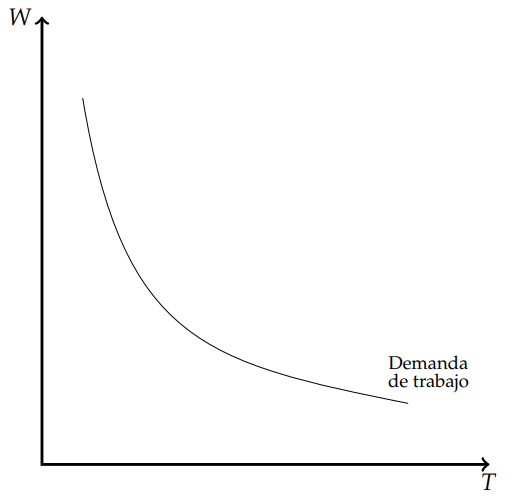
\includegraphics[scale=0.6]{../Figures/C34.1.png} 
\end{frame}


\begin{frame}{Mercado de trabajo: oferta de trabajo}
    \begin{itemize}
        \item ¿Cómo responde la oferta de trabajo ante un cambio en los salarios?
        \begin{itemize}
            \item Shock temporario $\Rightarrow$ la oferta de trabajo aumenta
            \begin{itemize}
                \item No llego a sentirme más rico por un trabajo extra
                \item El efecto sustitución es más fuerte que el efecto ingreso
            \end{itemize}
            \item Shock permanente $\Rightarrow$ la oferta de trabajo no se modifica
            \begin{itemize}
                \item Se compensan ambos efectos
                \item La gente siente que necesita trabajar más (ES) 
                \item Pero también se siente más rica y trabaja menos (EI)
            \end{itemize}
            \item Un ejemplo que ilustra esto último: desde la época medieval hemos trabajado aprox unas 8 horas por día
        \end{itemize}
    \end{itemize}
\end{frame}

\begin{frame}{Mercado de trabajo: oferta de trabajo}
    \centering
    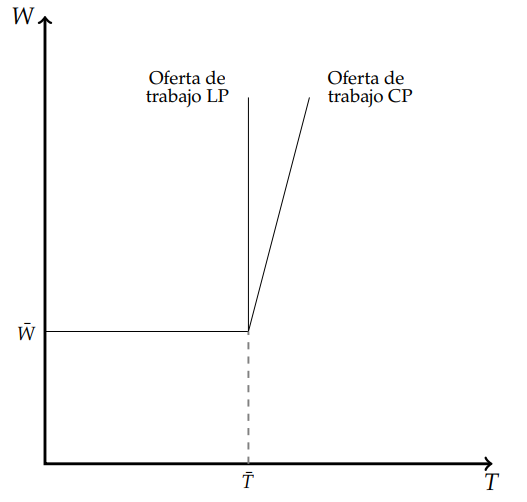
\includegraphics[scale=0.6]{../Figures/C34.4.png}
\end{frame}

\begin{frame}{Mercado de trabajo: el equilibrio}
\begin{itemize}
    \small
    \item Dijimos la clase pasada que este mercado diferencia a los clásicos de los keynesianos.
    \item Si el salario está por encima de su valor de equilibrio ($W^{*}$) habrá desempleo.
    \item El desempleo es precisamente la situación en la que hay más gente que \textbf{quiere trabajar} que los puestos de trabajo que hay para contratarlos.
\end{itemize}
    \centering
    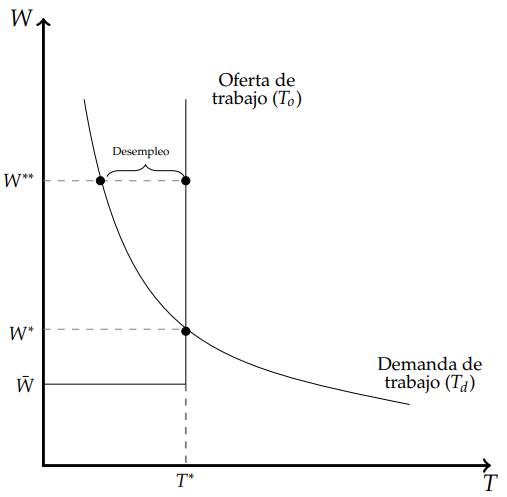
\includegraphics[scale=0.5]{../Figures/C34.5.png}
\end{frame}


\begin{frame}{La visión de los Clásicos}
    \begin{itemize}
        \item Según esta visión el mercado de trabajo siempre está en equilibrio:
        \begin{itemize}
        \item Es decir que el $W^{*}$ es el de equilibrio
        \item Si no lo está, por alguna rigidez, surge un mercado informal que compensa
        \item De esta manera, el nivel de actividad es siempre el de pleno empleo
        \item Y la oferta agregada es vertical
        \end{itemize}
        \item ¿Qué explica el desempleo?
        \begin{itemize}
            \item Desempleo friccional
            \begin{itemize}
                \item Regulaciones laborales
                \item Búsqueda de empleo
                \item Seguros de desempleo
            \end{itemize}
            \item Salarios de reserva altos
            \item Problemas de medición
        \end{itemize}
    \end{itemize}
\end{frame}

\begin{frame}{La visión Keynesiana}
    El mercado de trabajo \textbf{no siempre} está en equilibrio:
    \begin{itemize}
        \item ¿Por qué puede el salario real permanecer fuera del equilibrio?
        \begin{itemize}
            \item Rigideces nominales
            \item Sindicatos
            \item Contratos de largo plazo
            \item Salarios de eficiencia
       \end{itemize}
    \end{itemize}
    \centering
    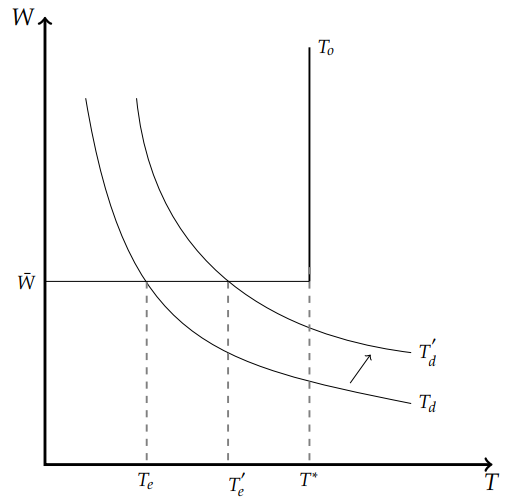
\includegraphics[scale=0.4]{../Figures/C34.7.png}
\end{frame}

\begin{frame}{Midiendo el desempleo}
    \begin{itemize}
        \item La EPH (Encuesta Permanente de Hogares) es una de las fuentes de datos más importantes
        \item Caracterizamos a las personas en activas o inactivas:
        \begin{itemize}
            \item Población Económicamente Activa (PEA): personas que trabajan o \textbf{buscan trabajo}.
            \item Población Económicamente Inactiva: personas que no trabajan y no buscan trabajo (incluye niños, jubilados, entre otros "inactivos").
        \end{itemize}
        \item Movimiento en el desempleo van a estar influenciados no solo por movimientos en empleados sino por quienes salen o entren de la inactividad.
    \end{itemize}
\end{frame}


\begin{frame}{Indicadores básicos del mercado laboral}
    \[ \text {\textit{Tasa de desempleo}} = \frac{Desempleados}{\text{PEA}} \]
    
    \dangersignw Puede variar por: 
    \begin{itemize}
        \item Cambios en el número de desempleados
        \item Cambios en la fuerza laboral (PEA)
    \end{itemize}
    \[ \text {\textit{Tasa de empleo}} = \frac{Empleados}{\text{Población}} \]

    \[ \text {\textit{Tasa de participación}} = \frac{PEA}{\text{Población}} \]
\end{frame}

\begin{frame}{La tasa de desempleo en Argentina durante el COVID}
\centering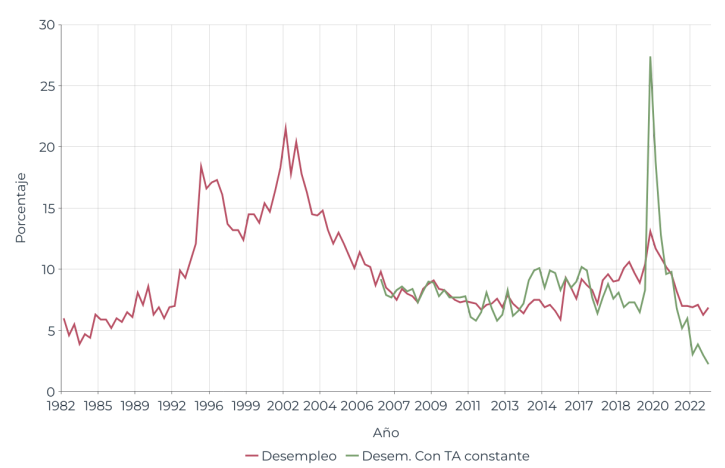
\includegraphics[width=11cm]{../Figures/C34.15.png}
\end{frame}

\begin{frame}{La decisión de actividad}
    \begin{itemize}
        \item La decisión de buscar trabajo es una decisión de actividad.
        \item Como sabemos buscar trabajo incrementa la oferta laboral.
        \item ¿Qué afecta el interés por incrementar esta oferta más que el salario?
        \begin{itemize}
            \item Seguros de desempleo
            \item Costos de búsqueda
            \item Expectativas
            \item ¿Otros?
        \end{itemize}
    \end{itemize}
\end{frame}

\begin{frame}{El mercado de trabajo en la Argentina}
\centering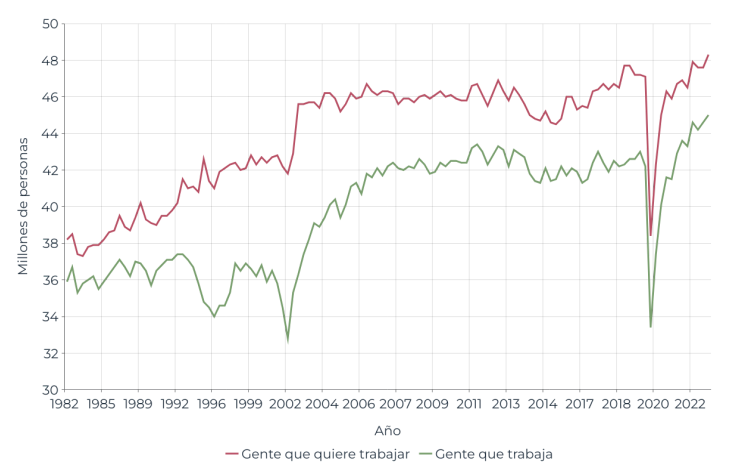
\includegraphics[width=11cm]{../Figures/C34.17.png}
\end{frame}

\begin{frame}{El mercado de trabajo en la Argentina}
\centering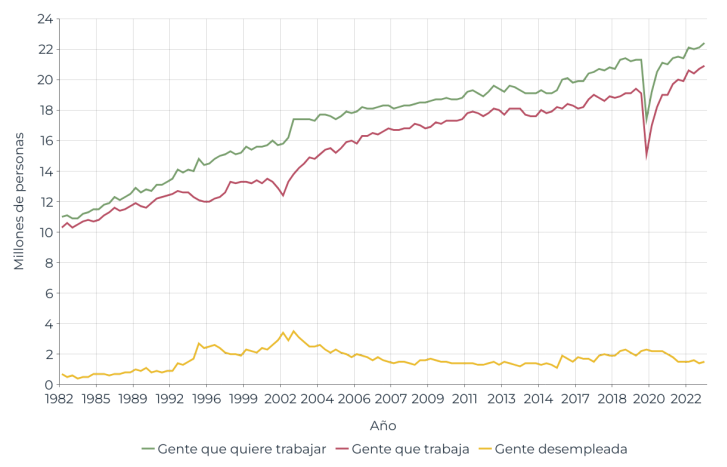
\includegraphics[width=11cm]{../Figures/C34.18.png}
\end{frame}

\begin{frame}{El mercado de trabajo en la Argentina}
\centering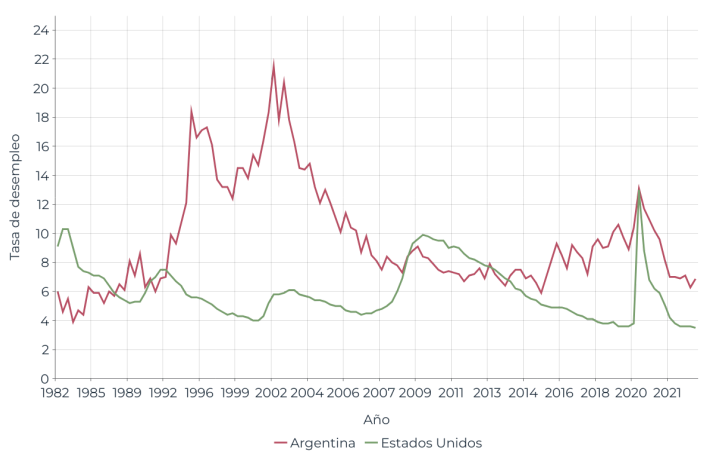
\includegraphics[width=11cm]{../Figures/C34.19.png}
\end{frame}

\end{document}